% !TEX root = ../main.tex

\section{Testing}
\label{sec:testing}

\noindent\textit{The numbers below are preliminary, from the best checkpoint of a manually-interrupted, not-yet-converged run (\secref{subsec:selection}); they stand in for the complete result set (full training curves and qualitative comparisons) to be added once final runs are completed.}

\subsection{Quantitative comparison}
\label{subsec:quant}

\tab{tab:results} reports the metrics of \secref{subsec:metrics} on MIT1003 for the best checkpoint of each model.

\begin{table}[t]
\centering
\caption{MIT1003 cross-dataset test results (best checkpoint, preliminary). $\downarrow$: lower is better, $\uparrow$: higher is better.}
\label{tab:results}
\begin{tabular}{@{}lcccc@{}}
\toprule
\textbf{Model} & $\mathcal{L}_{\mathrm{total}}\downarrow$ & KLD$\downarrow$ & CC$\uparrow$ & SIM$\uparrow$ \\
\midrule
v1.1 (CNN encoder)         & 7.6305 & 0.9229 & \textbf{0.6044} & \textbf{0.4809} \\
v2.0 (Swin-Tiny encoder)   & \textbf{7.5088} & 0.9436 & 0.5929 & 0.4609 \\
\bottomrule
\end{tabular}
\end{table}

\begin{figure}[t]
\centering
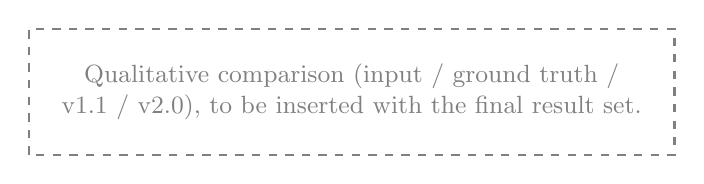
\begin{tikzpicture}
\draw[dashed, thick, gray] (0,0) rectangle (8.2,1.6);
\node[align=center, text width=7.4cm, font=\small, color=gray] at (4.1,0.8)
  {Qualitative comparison (input / ground truth / v1.1 / v2.0), to be inserted with the final result set.};
\end{tikzpicture}
\caption{Placeholder for the qualitative comparison figure.}
\label{fig:qual-placeholder}
\end{figure}

\subsection{Discussion}
\label{subsec:testdiscuss}

The two models are, at this stage, remarkably close: v2.0 reaches a marginally lower total loss, but v1.1 leads on all three individual metrics. Given how close the numbers are, we do not read this as a reliable ranking; it is consistent with our impression during development (\secref{subsec:v20-workflow}) that the pretrained Transformer encoder has not yet translated into a clear generalization advantage under the current training regime. We discuss possible explanations in \secref{sec:conclusions}.
